% This is "sig-alternate.tex" V2.0 May 2012
% This file should be compiled with V2.5 of "sig-alternate.cls" May 2012
%
% This example file demonstrates the use of the 'sig-alternate.cls'
% V2.5 LaTeX2e document class file. It is for those submitting
% articles to ACM Conference Proceedings WHO DO NOT WISH TO
% STRICTLY ADHERE TO THE SIGS (PUBS-BOARD-ENDORSED) STYLE.
% The 'sig-alternate.cls' file will produce a similar-looking,
% albeit, 'tighter' paper resulting in, invariably, fewer pages.
%
% ----------------------------------------------------------------------------------------------------------------
% This .tex file (and associated .cls V2.5) produces:
%       1) The Permission Statement
%       2) The Conference (location) Info information
%       3) The Copyright Line with ACM data
%       4) NO page numbers
%
% as against the acm_proc_article-sp.cls file which
% DOES NOT produce 1) thru' 3) above.
%
% Using 'sig-alternate.cls' you have control, however, from within
% the source .tex file, over both the CopyrightYear
% (defaulted to 200X) and the ACM Copyright Data
% (defaulted to X-XXXXX-XX-X/XX/XX).
% e.g.
% \CopyrightYear{2007} will cause 2007 to appear in the copyright line.
% \crdata{0-12345-67-8/90/12} will cause 0-12345-67-8/90/12 to appear in the copyright line.
%
% ---------------------------------------------------------------------------------------------------------------
% This .tex source is an example which *does* use
% the .bib file (from which the .bbl file % is produced).
% REMEMBER HOWEVER: After having produced the .bbl file,
% and prior to final submission, you *NEED* to 'insert'
% your .bbl file into your source .tex file so as to provide
% ONE 'self-contained' source file.
%
% ================= IF YOU HAVE QUESTIONS =======================
% Questions regarding the SIGS styles, SIGS policies and
% procedures, Conferences etc. should be sent to
% Adrienne Griscti (griscti@acm.org)
%
% Technical questions _only_ to
% Gerald Murray (murray@hq.acm.org)
% ===============================================================
%
% For tracking purposes - this is V2.0 - May 2012

\documentclass{sig-alternate}

% ===============================================================
%    My Commands
    \newcommand{\bi}{\begin{itemize}}
    \newcommand{\ei}{\end{itemize}}
    \newcommand{\be}{\begin{enumerate}}
    \newcommand{\ee}{\end{enumerate}}
    \newcommand{\ii}{\item}
    \newtheorem{Def}{Definition}
    \newtheorem{Lem}{Lemma}

    \usepackage{algorithm}
    \usepackage{algorithmicx}
    \usepackage{algpseudocode}

    \usepackage{graphicx}
    \graphicspath{%
        {converted_graphics/}% inserted by PCTeX
        {./images/}% inserted by PCTeX
    }

\usepackage{times}
% ===============================================================

\begin{document}
%
% --- Author Metadata here ---
\conferenceinfo{\textit{Middleware 2014 Industry Track,}}{December 8-12, Bordeaux, France}
\CopyrightYear{2014} % Allows default copyright year (20XX) to be over-ridden - IF NEED BE.
%\crdata{0-12345-67-8/90/01}  % Allows default copyright data (0-89791-88-6/97/05) to be over-ridden - IF NEED BE.
% --- End of Author Metadata ---

\title{PCS: Persistent Collaboration Sessions in Multiscreen Environments}
%\subtitle{[Extended Abstract]
%\titlenote{A full version of this paper is available as
%\textit{Author's Guide to Preparing ACM SIG Proceedings Using
%\LaTeX$2_\epsilon$\ and BibTeX} at
%\texttt{www.acm.org/eaddress.htm}}}

%
% You need the command \numberofauthors to handle the 'placement
% and alignment' of the authors beneath the title.
%
% For aesthetic reasons, we recommend 'three authors at a time'
% i.e. three 'name/affiliation blocks' be placed beneath the title.
%
% NOTE: You are NOT restricted in how many 'rows' of
% "name/affiliations" may appear. We just ask that you restrict
% the number of 'columns' to three.
%
% Because of the available 'opening page real-estate'
% we ask you to refrain from putting more than six authors
% (two rows with three columns) beneath the article title.
% More than six makes the first-page appear very cluttered indeed.
%
% Use the \alignauthor commands to handle the names
% and affiliations for an 'aesthetic maximum' of six authors.
% Add names, affiliations, addresses for
% the seventh etc. author(s) as the argument for the
% \additionalauthors command.
% These 'additional authors' will be output/set for you
% without further effort on your part as the last section in
% the body of your article BEFORE References or any Appendices.

\numberofauthors{3} %  in this sample file, there are a *total*
% of EIGHT authors. SIX appear on the 'first-page' (for formatting
% reasons) and the remaining two appear in the \additionalauthors section.
%
\author{
% You can go ahead and credit any number of authors here,
% e.g. one 'row of three' or two rows (consisting of one row of three
% and a second row of one, two or three).
%
% The command \alignauthor (no curly braces needed) should
% precede each author name, affiliation/snail-mail address and
% e-mail address. Additionally, tag each line of
% affiliation/address with \affaddr, and tag the
% e-mail address with \email.
%
% 1st. author
\alignauthor
Sung-Soo Kim\\
       \affaddr{ETRI}\\
%       \affaddr{218 Gajeong-ro, Yuseong-gu}\\
       \affaddr{Daejeon, South Korea}\\
       \email{sungsoo@etri.re.kr}
% 2nd. author
\alignauthor
Chunglae Cho\\
       \affaddr{ETRI}\\
%       \affaddr{218 Gajeong-ro, Yuseong-gu}\\
       \affaddr{Daejeon, South Korea}\\
       \email{clcho@etri.re.kr}
% 3rd. author
\alignauthor 
Jongho Won\\
       \affaddr{ETRI}\\
%       \affaddr{218 Gajeong-ro, Yuseong-gu}\\
       \affaddr{Daejeon, South Korea}\\
       \email{jhwon@etri.re.kr}
%\and  % use '\and' if you need 'another row' of author names
% 4th. author
%\alignauthor Lawrence P. Leipuner\\
%       \affaddr{Brookhaven Laboratories}\\
%       \affaddr{Brookhaven National Lab}\\
%       \affaddr{P.O. Box 5000}\\
%       \email{lleipuner@researchlabs.org}
% 5th. author
%\alignauthor Sean Fogarty\\
%       \affaddr{NASA Ames Research Center}\\
%       \affaddr{Moffett Field}\\
%       \affaddr{California 94035}\\
%       \email{fogartys@amesres.org}
% 6th. author
%\alignauthor Charles Palmer\\
%       \affaddr{Palmer Research Laboratories}\\
%       \affaddr{8600 Datapoint Drive}\\
%       \affaddr{San Antonio, Texas 78229}\\
%       \email{cpalmer@prl.com}
}
% There's nothing stopping you putting the seventh, eighth, etc.
% author on the opening page (as the 'third row') but we ask,
% for aesthetic reasons that you place these 'additional authors'
% in the \additional authors block, viz.
%\additionalauthors{Additional authors: John Smith (The Th{\o}rv{\"a}ld Group,
%email: {\texttt{jsmith@affiliation.org}}) and Julius P.~Kumquat
%(The Kumquat Consortium, email: {\texttt{jpkumquat@consortium.net}}).}
%\date{30 July 1999}
% Just remember to make sure that the TOTAL number of authors
% is the number that will appear on the first page PLUS the
% number that will appear in the \additionalauthors section.

\maketitle
\begin{abstract}
Multiscreen devices create new opportunities and challenges for collaboration services.

In this paper, we propose a mobile middleware for symmetric collaboration among associated mobile applications in the same network environment. 
This paper focuses on the challenge of providing the seamless services. 
The proposed middleware supports seamless collaboration services by maintaining the collaboration session even if the user changes one of the smart devices which participate in the collaboration session. 
The application developer can implement the collaboration-based multiscreen services easy and fast by using major functions in the middle ware API, such as remote execution, session join, session invitation,  push migration and pull migration. 

The major advantages of the collaboration middleware are providing communication transparency and seamless collaboration service delivery regardless of the changes of physical device configurations for collaboration.

\end{abstract}

% A category with the (minimum) three required fields
\category{H.4}{Information Systems Applications}{Miscellaneous}
%A category including the fourth, optional field follows...
\category{D.2.8}{Software Engineering}{Metrics}[complexity measures, performance measures]

\terms{Middleware, Mobile Computing}

\keywords{ACM proceedings, \LaTeX, text tagging}

\section{Introduction}
In recent years, there has been an increased interest in smart applications. The main reason for this has been the realization that many diverse applications need a generic middleware for managing applications and their context information. In this paper, we describe the collaboration persistency. 

A Smart Home environment is a home equipped with sensors and activators of various types to monitor activities and movement, and to monitor risk situations, such as fire and smoke alarms. 

% Reference paper: Heterogeneity in mobile computing environments
The goal of mobile computing suggests including devices spanning the entire hardware spectrum. This augmentation includes the appliance of various use cases,  including both the pervasive access to mobile services and ubiquitous communication between mobile hosts. Hence, those application cases can be reduced to the basic demand of communication among heterogenous devices in heterogenous environment.
The ultimate goal of mobile middleware is to simplify the development of distributed applications.
The goal of mobile middleware is to provide abstractions that reduce development effort, to offer programming paradigms that make developing powerful mobile applications easier, and to foster interoperability between applications.
The essential role of middleware is to manage the complexity and heterogeneity of distributed infrastructures. 
On the one hand, middleware offers programming abstractions that hide some of the complexities of building a distributed application.
On the other hand, there is a complex software infrastructure that implements these abstractions.
Middleware is software that supports mediation between other software components, fostering interoperability between those components across heterogeneous platforms and varying resource levels.
Mobile agents put the action where the data are, allowing programs to move autonomously about a network in order to access remote resources.

Service discovery middleware extends the client-server (CS) paradigm to include dynamic discovery of services and more dynamic interaction between clients and services.
With service discovery middleware, developers can quickly develop highly dynamic client-server systems that are self-healing and support "plug and play" for individual components.
The concepts embodied in service discovery architectures are not completely new; however, service discovery frameworks standardize the environments in which to deploy highly dynamic, self-healing client-server architectures.

In the fields of broadcasting especially IPTV and content delivery, multiscreen video describes video content transformed into multiple formats, bit rates and resolutions for display on smart devices such as television, mobile phone, tablet computer and computer.

 In this paper, we propose a new mobile middleware to support the seamless collaboration services among heterogenous multiple mobile applications (or \textit{apps}) in various smart devices.
    To provide convincing the collaboration services in mobile computing environments, we describe the key requirements of multiscreen service systems as follows:
    \bi
    \ii \emph{Remote execution}: 
Latency is defined as the time between a player's action and the time the actual resulting game output on the player's screen. Since computer games are highly interactive, extremely low latency has to be achieved.
%    In case of the first-person shooting (FPS) game, the threshold of latency is below 100 msec
    The interaction delay in the games should be kept below 80ms in order to guarantee suitable user responsiveness.
    \ii \emph{Collaboration}: 
In order to provide a high-quality video (above 720p) interactively, data shall be reduced as much as possible but keeping quality. However, video encoding is computationally quite demanding.
    \ii \emph{Mobility}: 
In the case of network congestion, the network problems like increased latency, jitter, and packet losses distribute evenly on all competing traffic. However, the quality can be enhanced using quality of service (QoS) technologies to giver higher priority to game traffic in the network bottlenecks \cite{Jurgelionis:2010}.
    \ii \emph{Synchronization}: 
Since the servers of cloud-based gaming service system have high-performance CPUs and GPUs, the operating costs for the servers are quite expensive. So, it is necessary to develop the optimization technologies to minimize power consumption and network bandwidth \cite{Perlman:2009}.
%    Also, the dedicated hardware and software for video encoding and streaming can allow users to share common resources.
\ei

\noindent
\textbf{Motivation:} In this paper, .....

\noindent
\textbf{Our contributions:}

The rest of the paper is organized as follows.
    We briefly survey previous work on Gaming on Demand (GoD), parallel rendering and video encoding for the multiscreen services in Section \ref{sc:RelatedWork}.
    Section \ref{sc:Architecture} describes the proposed the system architecture and the core systems in our system.
    We explain implementation details of our multi-view rendering algorithm and describe the performance result in Section \ref{sc:Implementation}.
    In Section \ref{sc:Comparison}, we compare our system and algorithm with prior GPU-based algorithms and highlight some of the benefits.
    Finally, we discuss future work and conclude in Section \ref{sc:Conclusion}.

\section{Related Work}
\label{sc:RelatedWork}
In this section, we give a brief overview of related work on the middleware for mobile computing and multiscreen services.
    We also highlight many technical characteristics of multiscreen user experience technology.\\

Many researchers agree in handling heterogeneity by employing middleware solutions.
The key idea behind the middleware approaches is to position the middleware layer between the application layer at the top and the heterogeneous environments such as hardware and operating systems at the bottom. 

\section{System Architecture}
    \label{sc:Architecture}
    In this section, we describe the proposed system architecture for the multiscreen-based collaboration services.
    Our architecture consists of two major systems such as the proposed \textit{middleware} for smart devices and \textit{N-screen service cloud} as shown in Fig. \ref{fig:architecture}. Also, our middleware decomposes into 2 layers;  the \textit{N-screen application library} and \textit{collaboration agent}.  

\subsection{System Overview}

    \begin{figure}[htb] % float placement: (h)ere, page (t)op, page (b)ottom, other (p)age
    \centering
    \includegraphics[width=8.5cm,keepaspectratio]{systemarchitecture}
    \caption{Our system architecture}
    \label{fig:architecture}
    \end{figure}

    \begin{figure}[htb] % float placement: (h)ere, page (t)op, page (b)ottom, other (p)age
    \centering
    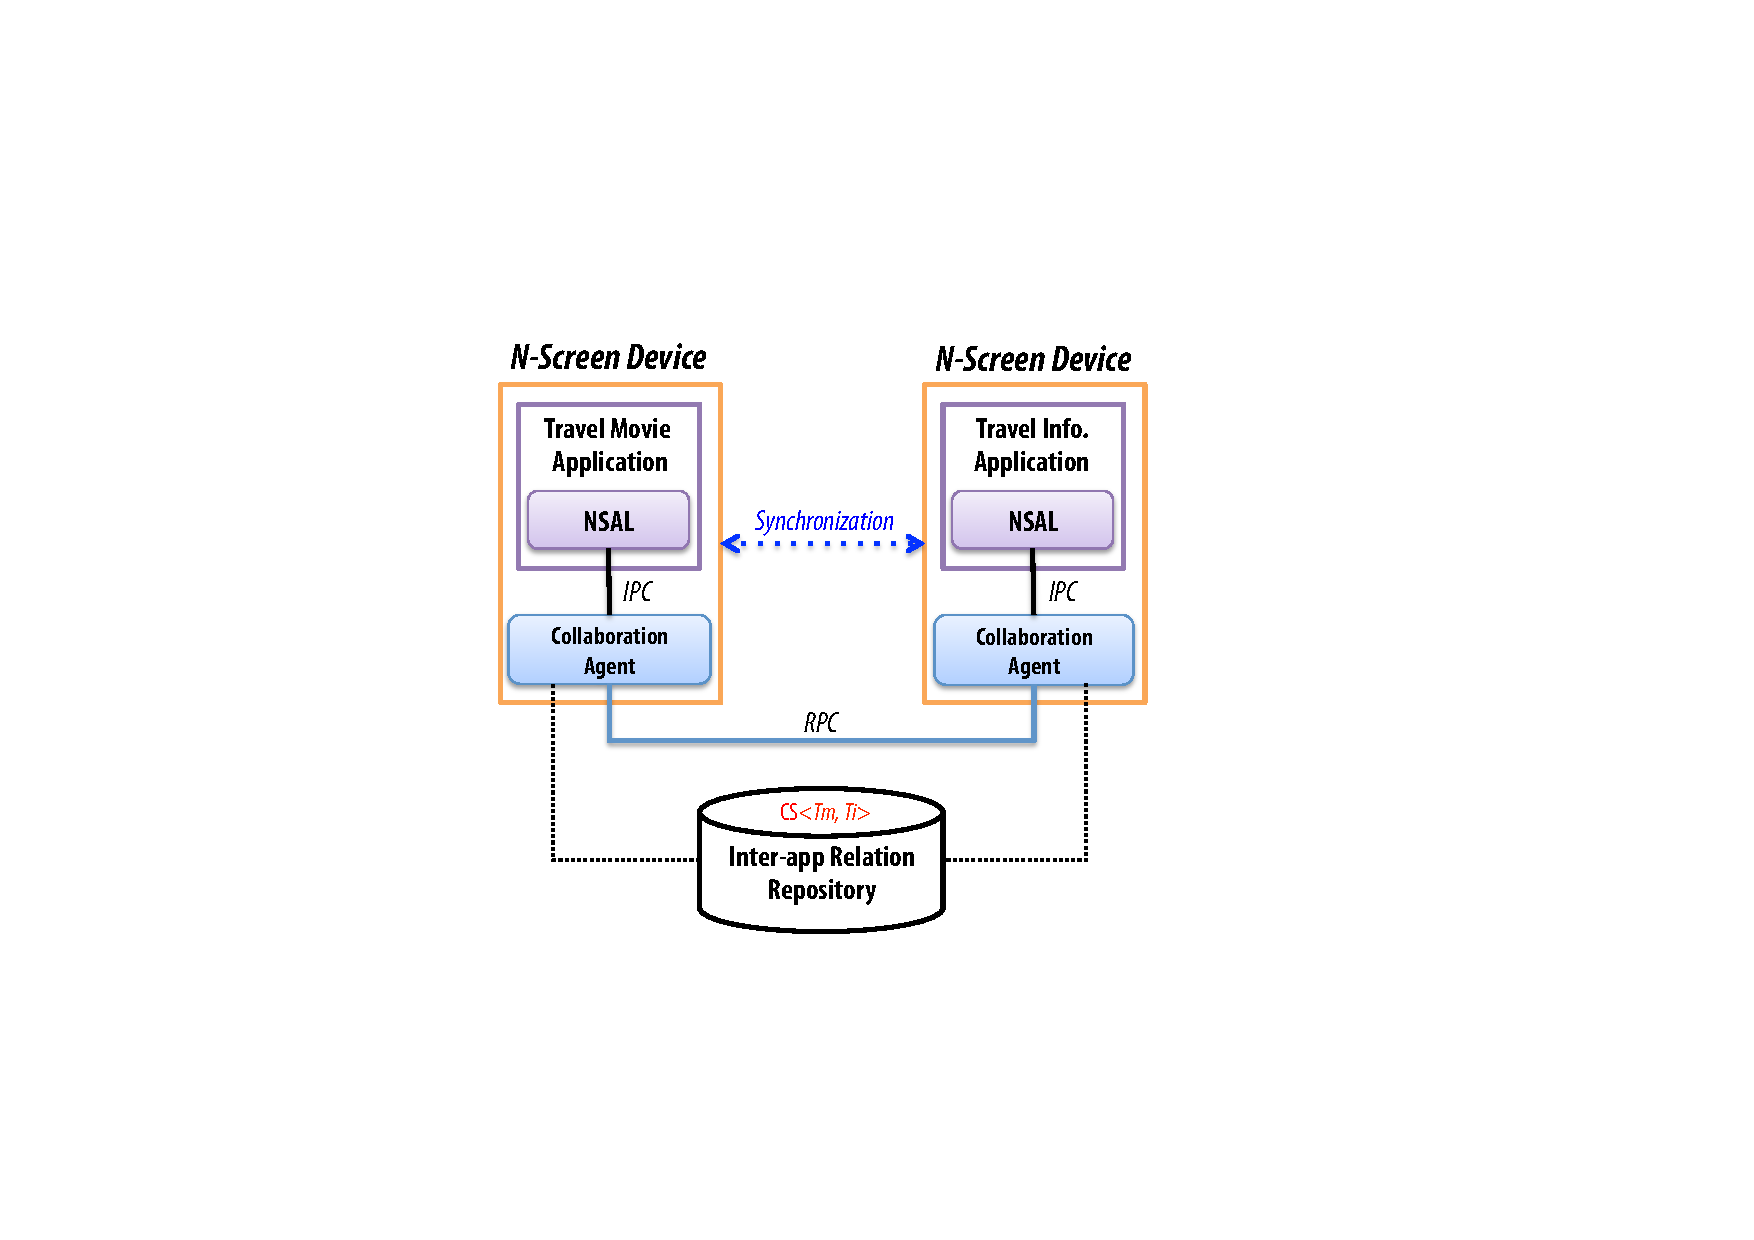
\includegraphics[width=5.5cm,keepaspectratio]{basicmodel}
    \caption{The CA block architecture}
    \label{fig:basicmodel}
    \end{figure}

\subsection{Definitions}
% Formal definitions and notations
N-Screen Devices

Logical Application

Physical Application

Collaboration Session

  Representation

    Inter-application relation schema

\subsection{N-Screen Application Library}
    \begin{figure}[htb] % float placement: (h)ere, page (t)op, page (b)ottom, other (p)age
    \centering
    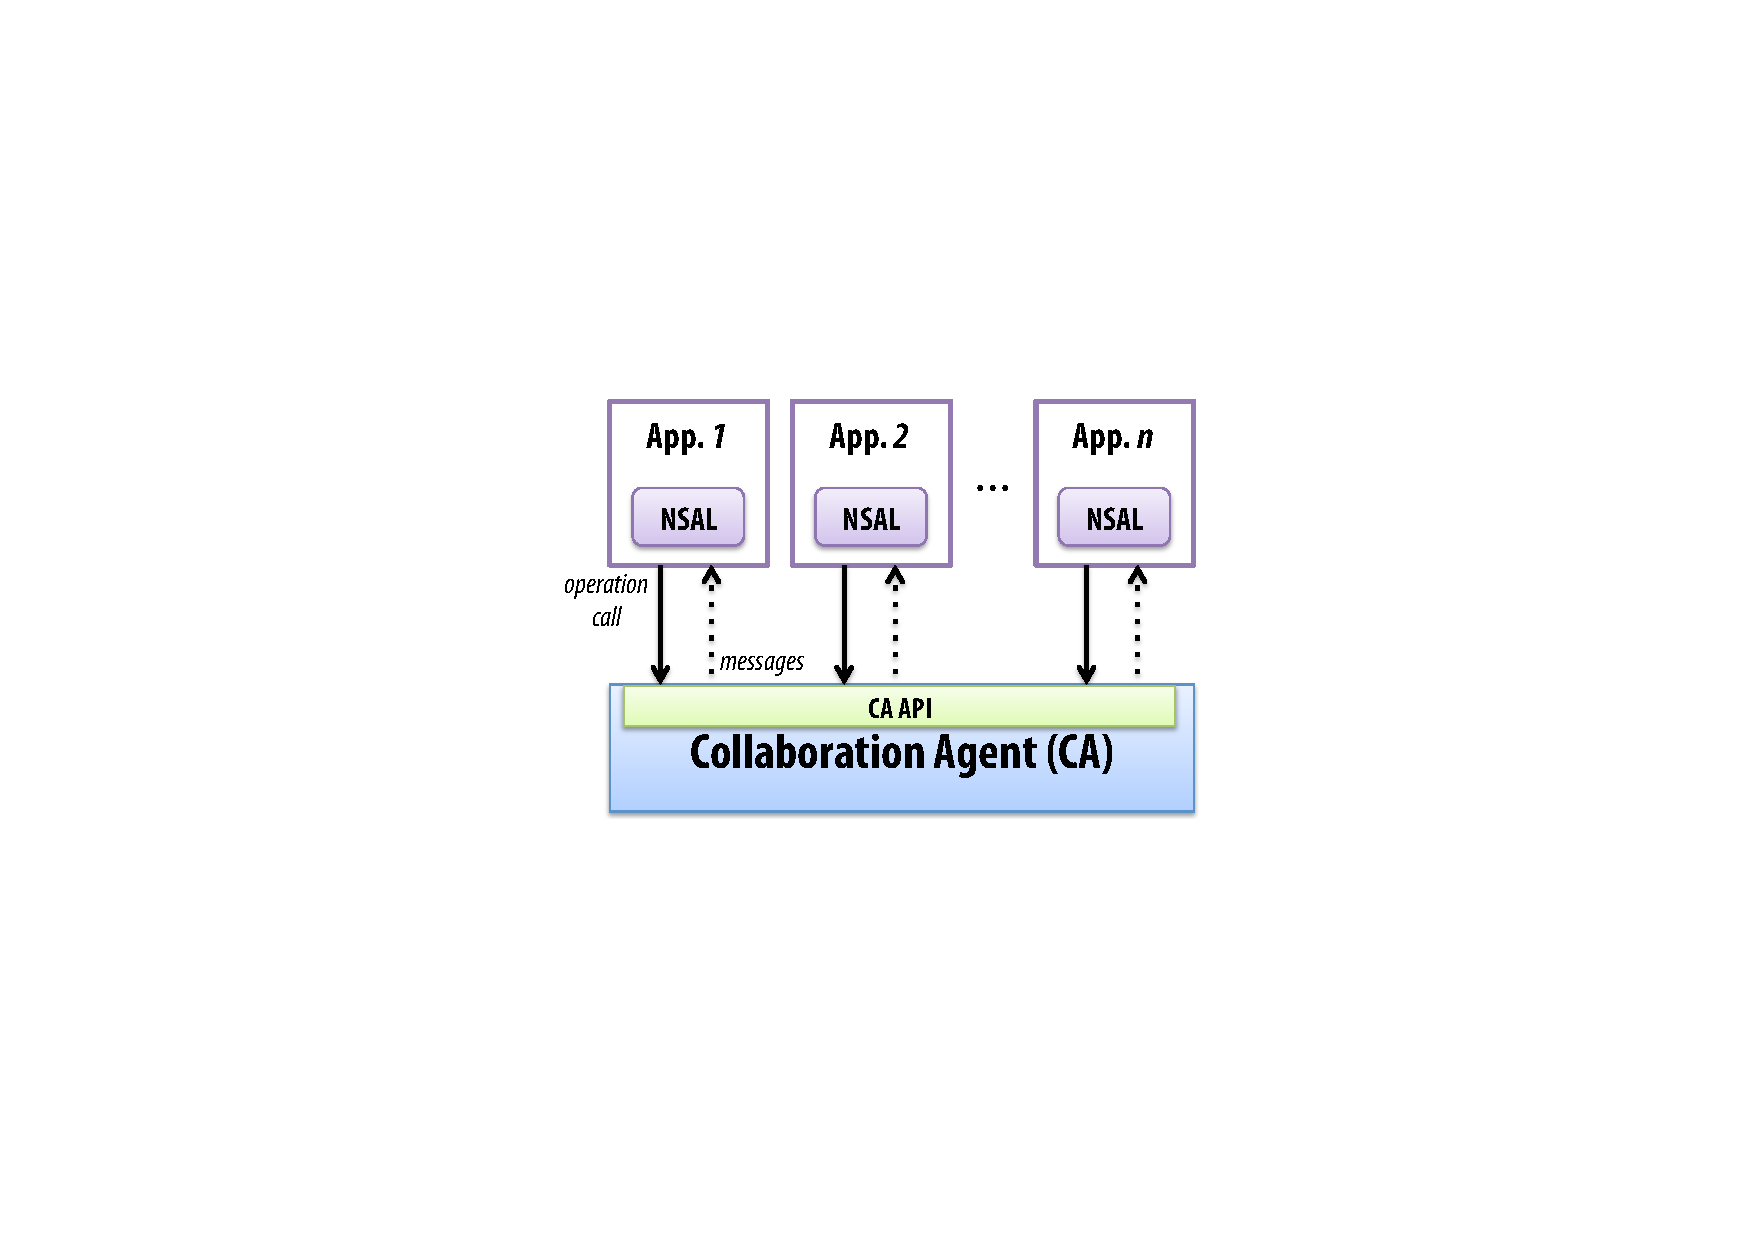
\includegraphics[width=5.5cm,keepaspectratio]{ca-api}
    \caption{An example workflow for collaboration session construction}
    \label{fig:ca-api}
    \end{figure}

\subsection{Collaboration Agent}

\noindent
\textbf{Major Operations:} 
\bi
\ii Service discovery
\ii Remote invocation
\ii Collaboration session join
\ii Collaboration session invitation
\ii Pull migration
\ii Push migration
\ii Synchronization
\ei

    \begin{figure}[htb] % float placement: (h)ere, page (t)op, page (b)ottom, other (p)age
    \centering
    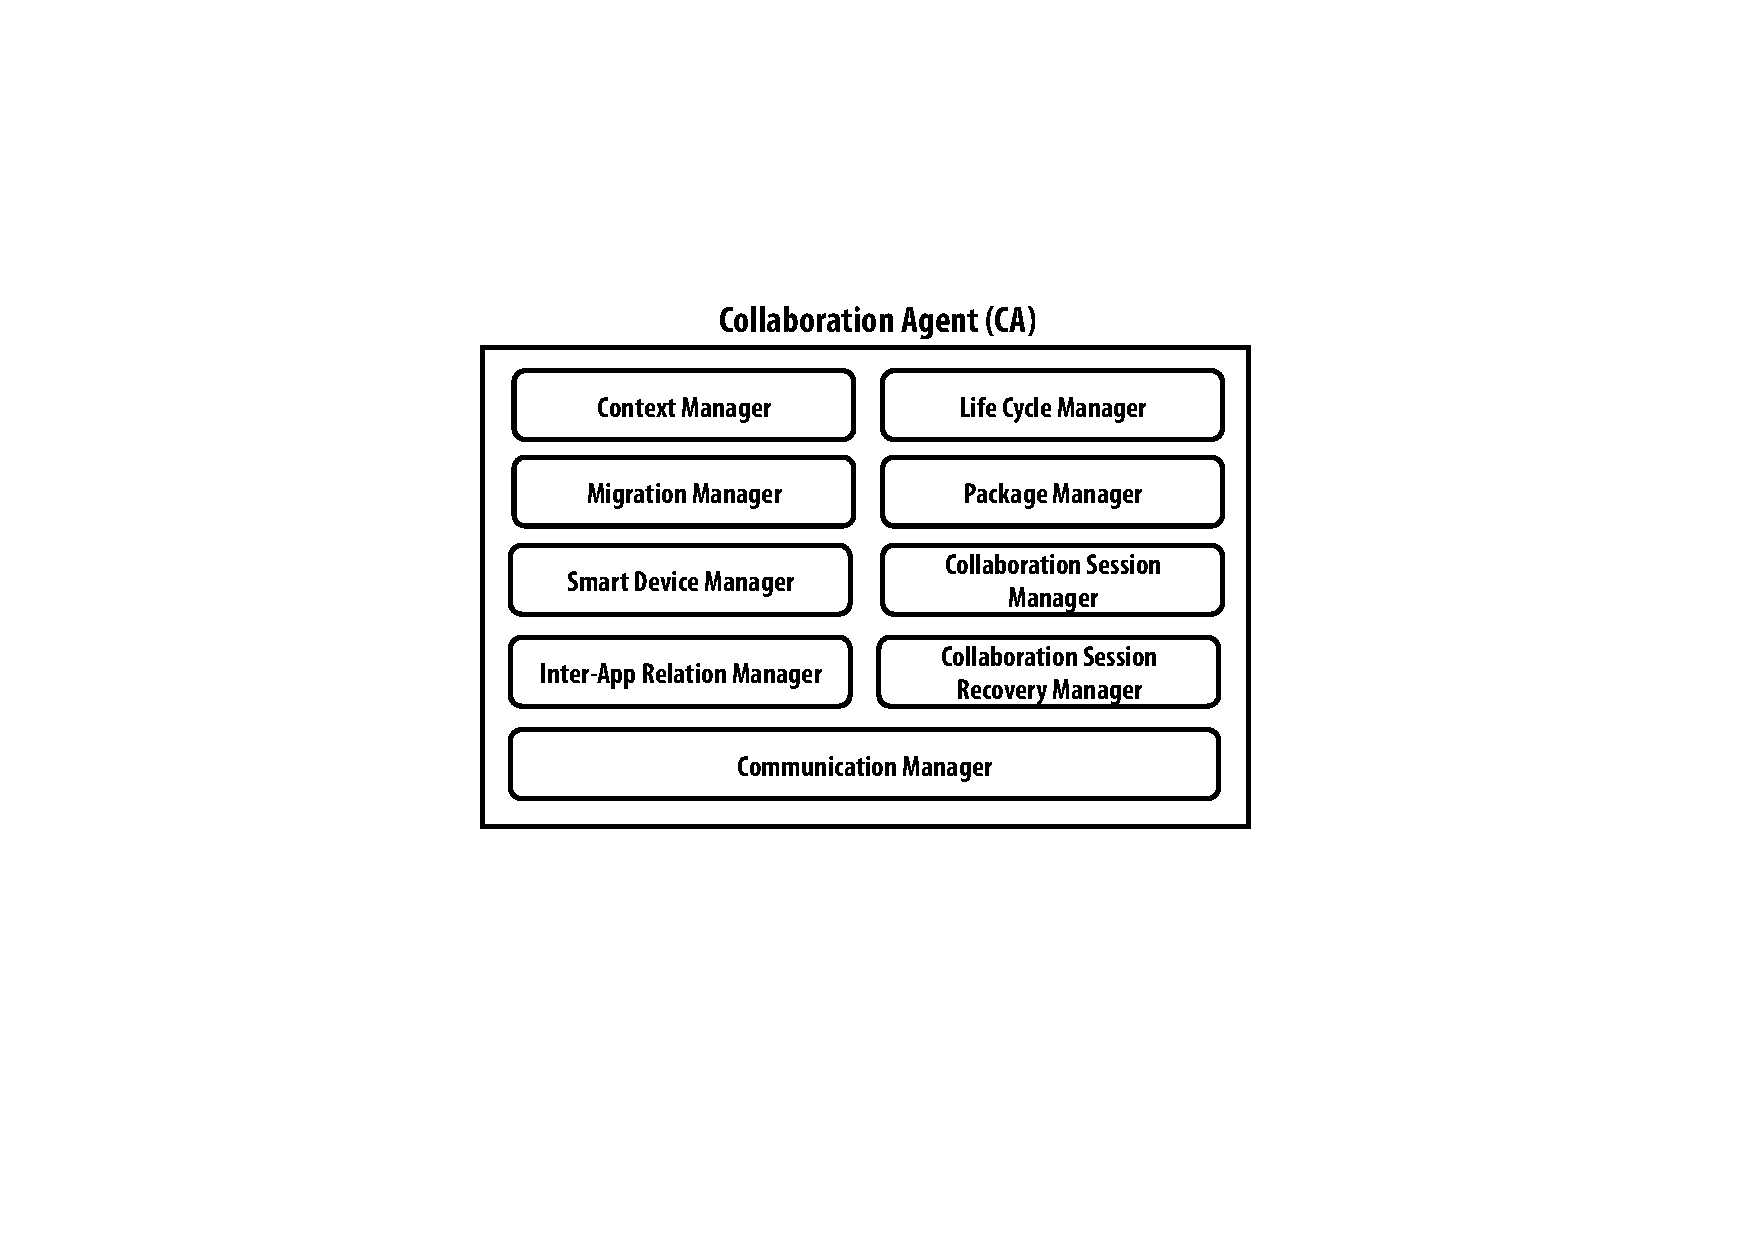
\includegraphics[width=7.5cm,keepaspectratio]{collaborationagent}
    \caption{The CA block architecture}
    \label{fig:collaborationagent}
    \end{figure}

\section{Collaboration Sessions}
The collaboration sessions are roughly analogous to social organizations.
The key approach to collaborating among the NSAL-based applications to organizing several interoperable applications into a group; we call this group a \textit{collaboration session}.
The purpose of introducing collaboration sessions is to allow n-screen applications to deal with collections of different smart apps as a single abstraction.

\subsection{Representation}

    \begin{figure}[htb] % float placement: (h)ere, page (t)op, page (b)ottom, other (p)age
    \centering
    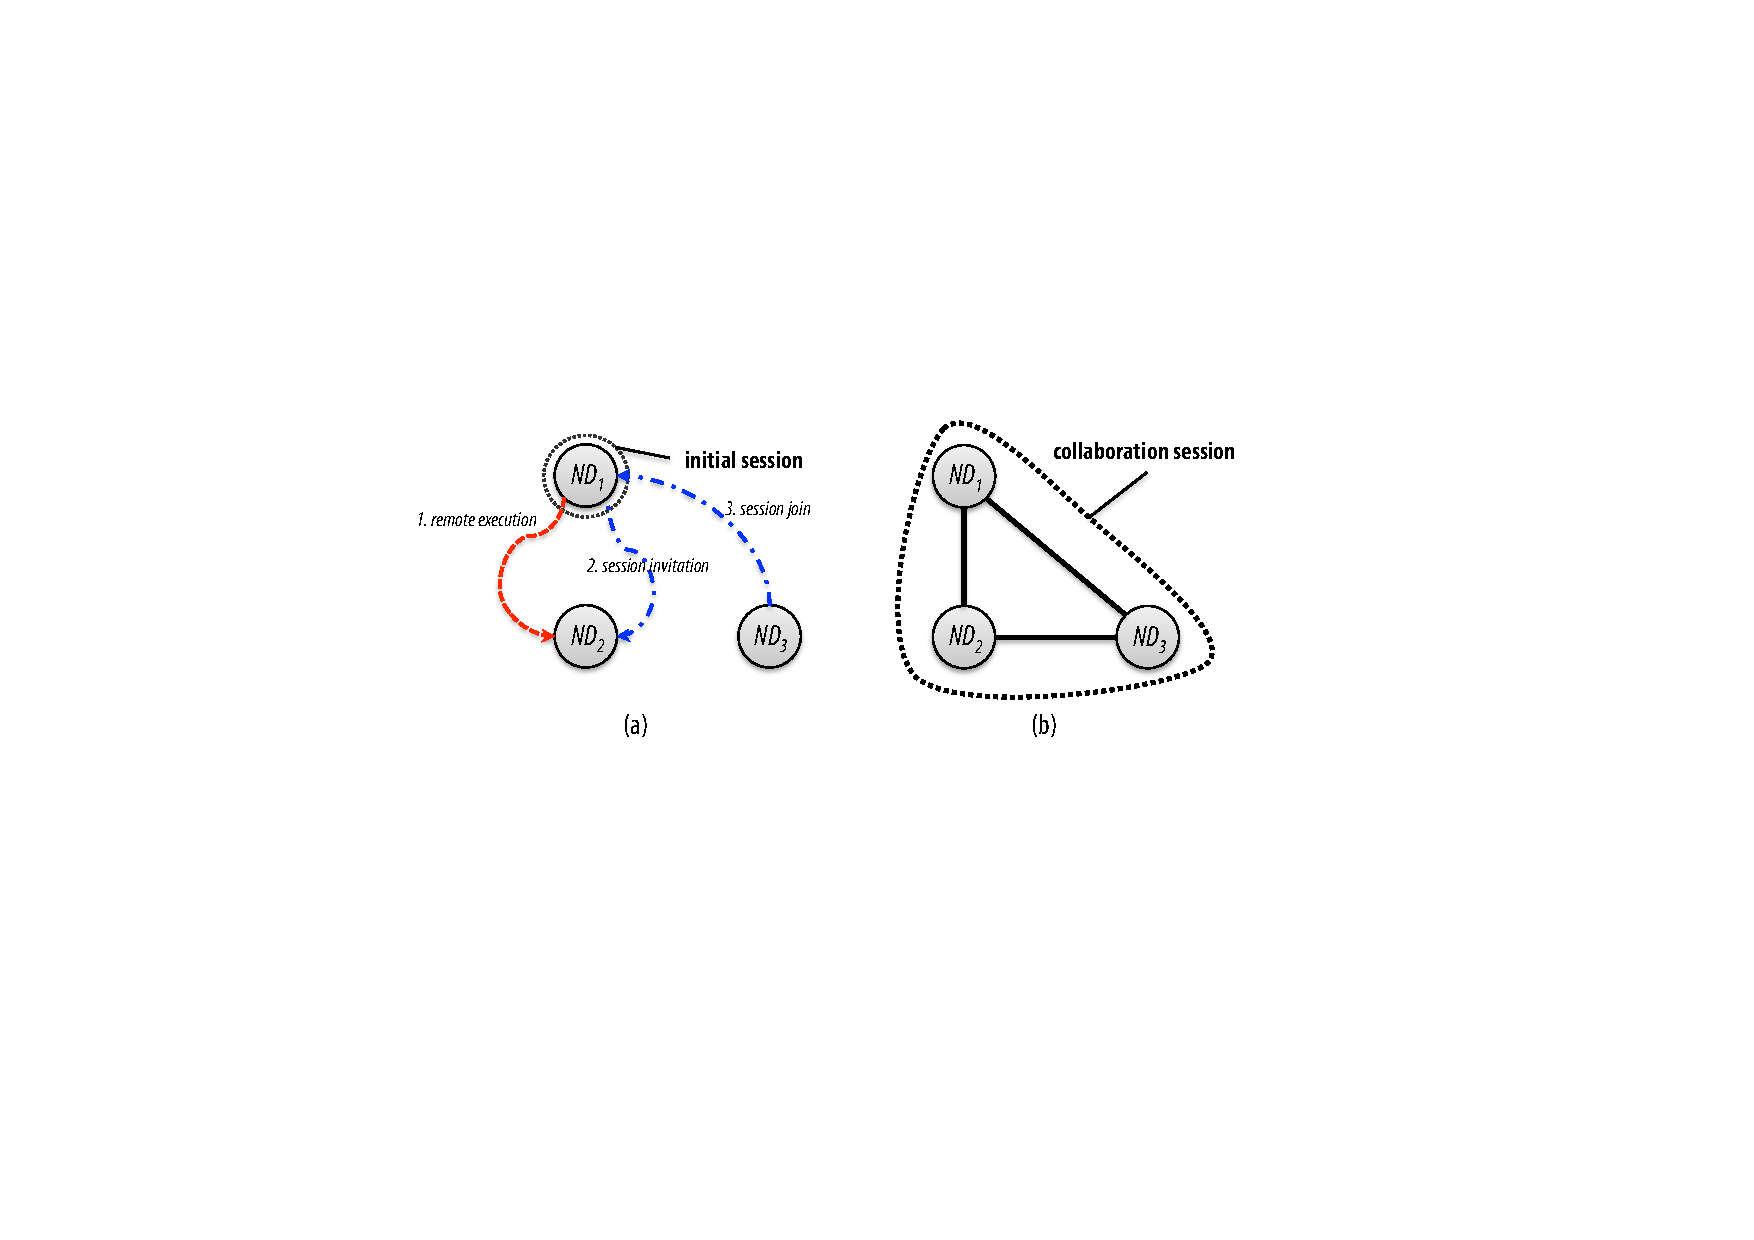
\includegraphics[width=8.5cm,keepaspectratio]{constructsession}
    \caption{An example workflow for collaboration session construction}
    \label{fig:constructsession}
    \end{figure}

\subsection{Persistency}

    \begin{figure}[htb] % float placement: (h)ere, page (t)op, page (b)ottom, other (p)age
    \centering
    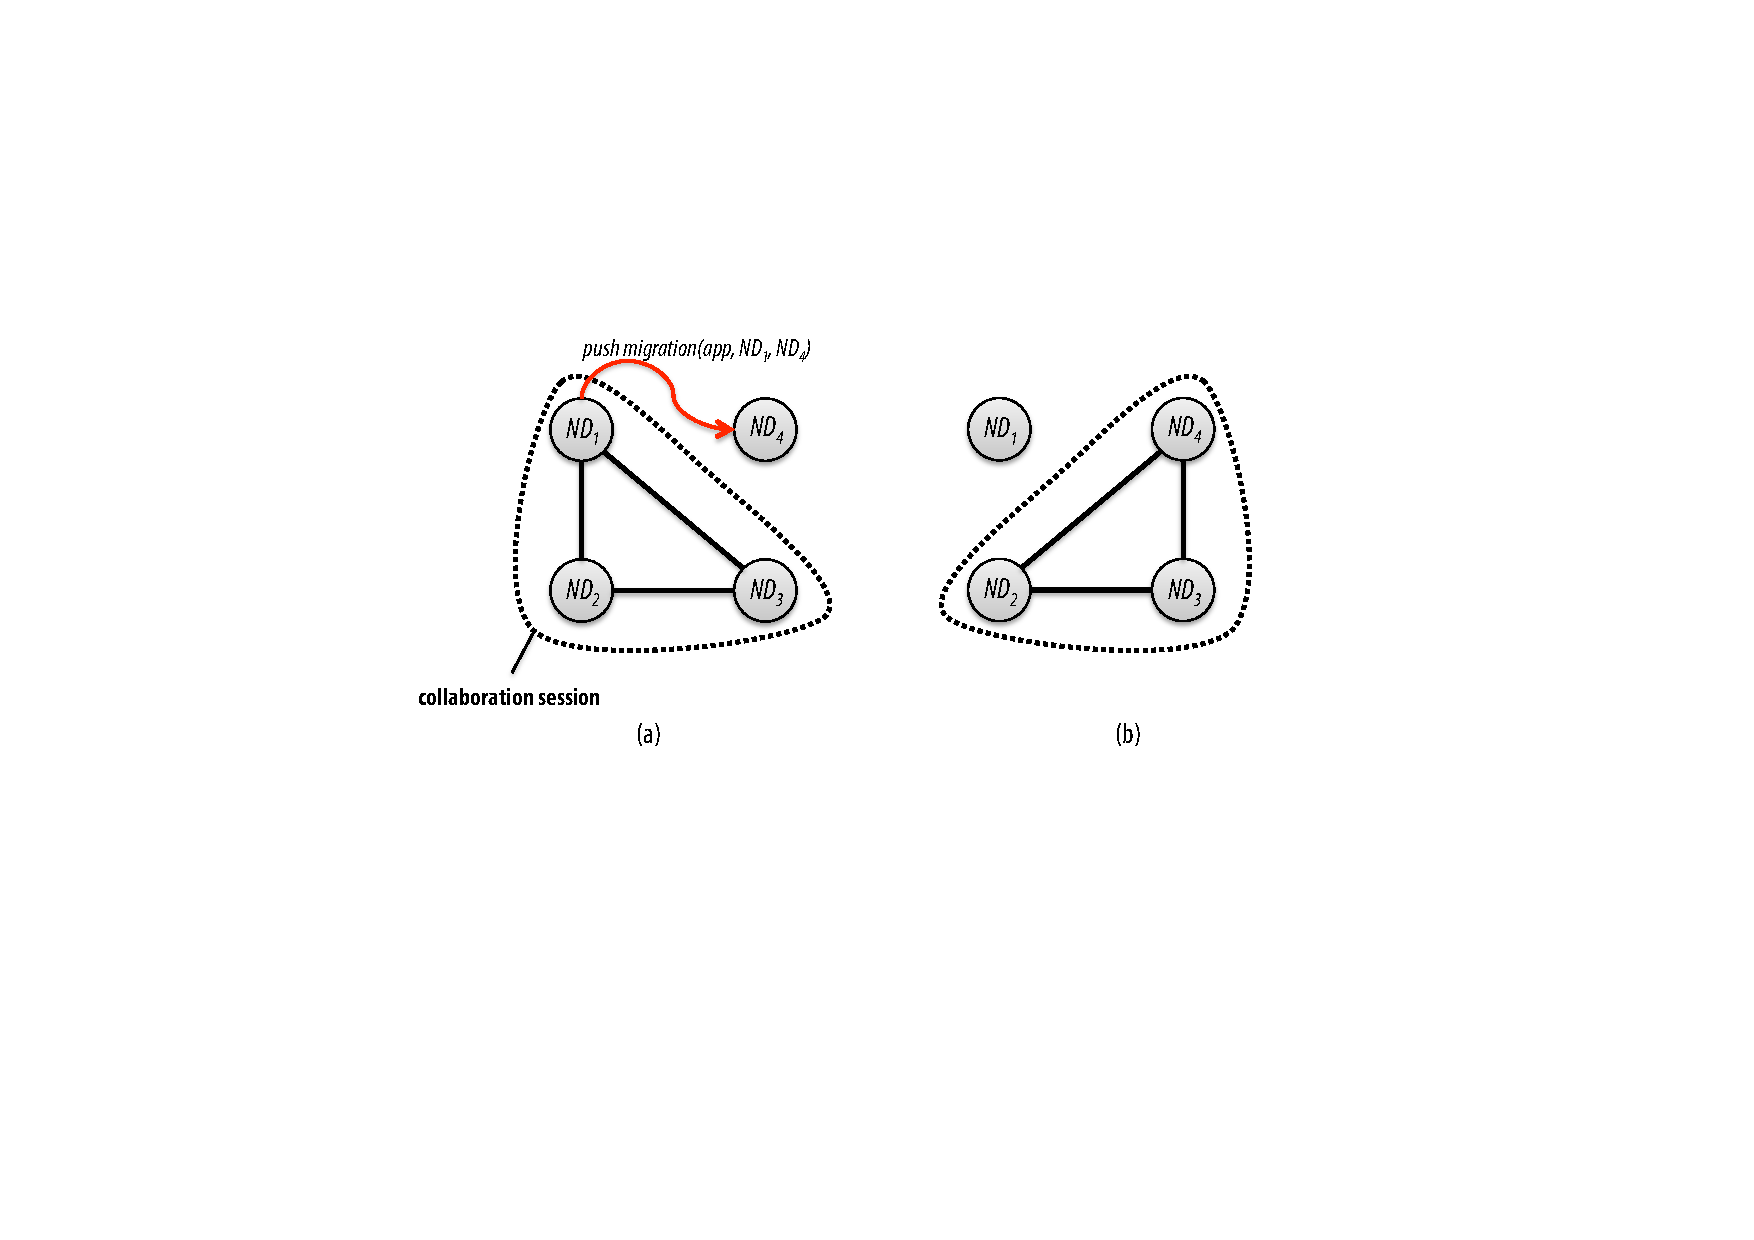
\includegraphics[width=8.5cm,keepaspectratio]{pushmigration}
    \caption{Collaboration session maintenance}
    \label{fig:pushmigration}
    \end{figure}

\subsection{Recovery}

\section{Implementation Details}
%NSAL
%  Brief Intro
%  Design Pattern
%  Major Classes
%CA
%  Brief Intro
%  Design Pattern
%  Major Classes
%Messaging Framework
%  Brief Intro
%  Design Patterns
%    Command Pattern
%    Object Factory Pattern
%    Class Diagram
%  Advantages

\section{Experimental Results}
%Experiments Setup
%  Home Network Configuration Diagram
%Travel Information Services
%Game Services
%Performance Results
%Discussion
%  Advantages
%  Limitations

    \noindent
    {\bf Analysis:} Our rendering system provides good performance scaling of multi-core CPUs for multi-view rendering.
    And the multi-view rendering algorithm maps well to the current GPUs and we have evaluated its performance on two different GPUs with different rendering resolution.
    Furthermore, it is relatively simple to combine the video encoding methods and optimizations in the streaming-based gaming service framework. This makes it possible to develop a more flexible GPU-based framework for the video encoding methods like H.264/AVC or ORBX which is GPU-based encoding schemes.\\

   \noindent
    {\bf Limitations:}
    Our approach has some limitations.
    First, we support the multi-view rendering for one multi-user game, since it is difficult to share the rendering resources in a GPU among different games. We believe that this can be resolved by using multi-GPUs.
    Secondly, our system performs directly rendering to the framebuffers on the server-side machines.
    However, in terms of efficient services in the cloud-based gaming, we should exploit the \emph{off-screen rendering} approaches and \emph{GPU virtualization} techniques.

\section{Conclusions}
    \label{sc:Conclusion}
    In this paper, we have presented a system architecture for the cloud-based gaming service and multi-view rendering.
%    Also, we have described a new technique for parallelized and distributed multi-view rendering.
    Our rendering system greatly improves utilization of hardware resources present in the system, allowing to utilize both multi-core CPUs and a GPU simultaneously.

    We found that the proposed system provide the multi-view rendering for different focal positions for each viewpoint with high visual quality.
    Moreover, our approach is flexible and maps well to current GPUs in terms of shared resources such as textures and shaders for rendering.
    In addition, we demonstrate that the proposed rendering system could prove to be scalable in terms of parallel rendering. So, we believe that our rendering system will provide high-quality with good performance for the cloud-based gaming services.

    There are many avenues for future work. It is possible to use new capabilities and optimizations to improve the performance of the video encoding especially H.264/AVC through the GPU-based implementation.
    Furthermore, we would like to develop algorithms for integrating the multi-view rendering with the video encoding in a GPU.
%    without a CPU-GPU I/O for the video encoding.


%ACKNOWLEDGMENTS are optional 
\section{Acknowledgments}
This work was supported by ETRI R\&D program ("\textit{Development of Big Data Platform for Dual Mode Batch Query Analysis}, 14ZS1400")
funded by the government of South Korea.

%
% The following two commands are all you need in the
% initial runs of your .tex file to
% produce the bibliography for the citations in your paper.
\bibliographystyle{abbrv}
\bibliography{sigproc}  % sigproc.bib is the name of the Bibliography in this case

\end{document}
